\documentclass[conference]{IEEEtran}

\usepackage{amsmath, amssymb}
\usepackage{graphicx}
\usepackage{float}
\usepackage{booktabs}
\usepackage{caption}

%------------------------------------------------
\begin{document}

\title{Identification and Control of a Propeller-Actuated Damped Pendulum (PADP)}

\author{
  \IEEEauthorblockN{
    Eric Castro Velásquez\IEEEauthorrefmark{1},
    Esteban Segura Garcia\IEEEauthorrefmark{1},
    Daniel Chavarria Garcia\IEEEauthorrefmark{1}
  }
  \vspace{2mm}
  \IEEEauthorblockA{
    \IEEEauthorrefmark{1}School of Electronics Engineering,
    Instituto Tecnológico de Costa Rica (ITCR), 30101 Cartago, Costa Rica \\
    \{ecastro, essegura, dachavarria\}@estudiantec.cr
  }
}

\maketitle

%================================================
%  ABSTRACT
%================================================
\begin{abstract}
% -----------------------------------------------------------------
% WHAT TO WRITE HERE (~80 words, be concise):
%   • One sentence: what system, what was done.
%   • Identification: 3 step-response experiments (0 to ~0.6 rad
%     equilibrium), parameter approximation + MATLAB SYSID toolbox
%     → 6 TFs total. Sample 3 discarded via statistical analysis.
%     Final plant = average of 4 valid TFs.
%   • Three continuous controllers designed: PID (IMC via SISOtool),
%     ISF-LQR, and I-PD (pole placement).
%   • Main result: ISF-LQR and I-PD met specs (ts ≤ 5 s, Mp ≤ 3 %);
%     PID showed the weakest transient performance.
% -----------------------------------------------------------------
This paper presents the experimental identification and closed-loop control of a propeller-actuated damped pendulum (PADP). Three step-response datasets were collected and processed using both manual parameter approximation and MATLAB's System Identification toolbox, yielding six candidate transfer functions. Statistical analysis identified one experiment as disturbance-affected and excluded it; the final plant model was obtained by averaging the four remaining models. Three continuous-time controllers were designed — a PID tuned via IMC in SISOtool, an integral state feedback regulator via LQR (ISF-LQR), and an I-PD by pole placement — and physically validated against a settling time of 5~s and maximum overshoot of 3\%. The ISF-LQR and I-PD controllers satisfied both specifications, while the PID exhibited the poorest transient response among the three.
\end{abstract}

%================================================
%  1. INTRODUCTION
%================================================
\section{Introduction}

The propeller-actuated damped pendulum (PADP) is an underactuated mechanical system whose
angular position is governed by the aerodynamic torque of a brushless motor and propeller
assembly. Around a fixed operating point, the nonlinear dynamics admit a linear second-order
underdamped approximation \cite{ogata2010}, making it a representative platform for comparing
control strategies under the design requirements of settling time $t_s \leq 5\,\text{s}$ and
maximum overshoot $M_p \leq 3\,\%$.

Plant identification was carried out using both parametric methods — extracting $\omega_n$ and
$\zeta$ from measured transient features — and data-driven fitting via MATLAB's \textit{ident}
toolbox \cite{ljung1999}. Statistical screening across repeated trials was applied to handle
noise and disturbances before model averaging.

Three control architectures were implemented and compared. A continuous PID tuned via Internal
Model Control (IMC) \cite{astrom2006}, a Linear Quadratic Regulator with augmented integral
state (ISF-LQR) \cite{anderson1990}, and an I-PD controller with pole placement \cite{visioli2006},
where the proportional and derivative terms act on the plant output to eliminate derivative kick
and reduce overshoot.


This paper reports the complete identification-to-validation cycle for the PADP. Section~\ref{sec:id}
covers parameter estimation and plant derivation. Section~\ref{sec:ctrl} details the controller
designs. Sections~\ref{sec:results} and~\ref{sec:disc} present and interpret the experimental
results against the design specifications.

%================================================
%  2. SYSTEM IDENTIFICATION
%================================================
\section{System Identification}
\label{sec:id}

\subsection{Experimental Setup and Data Acquisition}
% -----------------------------------------------------------------
% WHAT TO WRITE HERE:
%   • Briefly describe hardware: extruded-aluminium support, pivot
%     bearings, hollow aluminium tube, Hobbymate 2204 BLDC motor,
%     SimonK 20A ESC, GEMFAN 5045BNR 3-blade propeller.
%   • Sensor: USDigital E5 incremental quadrature encoder, 3600 CPR,
%     read every 20 ms → gain k = 2π/3600 rad/count (negative sign
%     to match pendulum direction).
%   • Actuation: PWM in OneShot125 mode, period 500 µs.
%   • Excitation: step of 1.7 units from 0, driving the pendulum to
%     its ~0.6 rad (≈34.4°) equilibrium point; data recorded for 40 s.
%   • Three independent trials under nominally identical conditions.
%   • Control platform: kit059-based board running PASCAL/AppLabControl.
% -----------------------------------------------------------------
The PADP platform consists of an extruded-aluminium support rigidly fixed to a wooden base. A hollow aluminium arm pivots on bearings at the top of the support and carries a Hobbymate~2204 brushless motor governed by a SimonK~20~A ESC fitted with a GEMFAN~5045BNR three-blade propeller. Angular position is measured by a USDigital~E5 incremental encoder (3600~CPR) coupled to the pivot shaft and sampled every 20~ms with a gain $k = 2\pi/3600$~rad/count. PWM actuation uses OneShot125 mode at a 500~µs period. Three independent experiments were conducted by applying a step input of 1.7~units from rest, establishing a steady-state operating point near $\theta_{eq} \approx 0.6$~rad ($\approx 34.4°$), and recording the angular response for 40~s.

% -----------------------------------------------------------------
% SUGGESTED FIGURE — three raw step responses overlaid:
% \begin{figure}[H]
%   \centering
%   \includegraphics[width=0.45\textwidth]{raw_responses.png}
%   \caption{Angular step responses for the three experimental trials.
%            The underdamped oscillation around the equilibrium point
%            is clearly visible in all three datasets.}
%   \label{fig:raw}
% \end{figure}
% -----------------------------------------------------------------

\subsection{Parameter Approximation}
% -----------------------------------------------------------------
% WHAT TO WRITE HERE:
%   • State that you applied the logarithmic decrement method from
%     Appendix A of the project guide to each of the 3 trials.
%   • Show the key equations used (δ, ζ, ω, ωn, K).
%   • Present the resulting (K, ζ, ωn) triplet for each trial in a
%     small inline table or as numbered equations.
%   • Conclude with the 3 TFs: G1_approx(s), G2_approx(s),
%     G3_approx(s).
% -----------------------------------------------------------------
The logarithmic decrement method~\cite{ogata2010} was
applied to each trial, yielding:

\begin{equation}
  \delta = \frac{\ln(y_0/y_i)}{i}, \quad
  \zeta  = \frac{\delta}{\sqrt{(2\pi)^2+\delta^2}}, \quad
  \omega_n = \frac{2\pi/T}{\sqrt{1-\zeta^2}}
  \label{eq:approx}
\end{equation}

yielding three second-order transfer functions of the prototype:
\begin{equation}
  G_i(s) = K_i\frac{\omega_{n,i}^2}{s^2+2\zeta_i\omega_{n,i}s+\omega_{n,i}^2}, \quad i=1,2,3
  \label{eq:tf_proto}
\end{equation}

% -----------------------------------------------------------------
% SUGGESTED TABLE — approximation results (3 trials):
 \begin{table}[H]
   \centering
   \caption{Parameters estimated by the logarithmic decrement method}
   \begin{tabular}{cccc}
     \toprule
     Trial & $K$ & $\zeta$ & $\omega_n$ (rad/s) \\
     \midrule
     1 & 0.338 & 0.032 & 3.9292 \\
     2 & 0.340 & 0.035 & 3.9294 \\
     3 & 0.423 & 0.033 & 3.9291 \\
     \bottomrule
   \end{tabular}
   \label{tab:approx}
 \end{table}
% -----------------------------------------------------------------

\subsection{MATLAB System Identification}
% -----------------------------------------------------------------
% WHAT TO WRITE HERE:
%   • Briefly describe the ident workflow: import time-series data,
%     select TF prototype of order 2 (underdamped poles), run
%     prediction-error minimization, report best-fit (%) for each trial.
%   • Present the three resulting TFs: G1_SI(s), G2_SI(s), G3_SI(s).
%   • Comment qualitatively on agreement / disagreement with the
%     approximation results above.
% -----------------------------------------------------------------
MATLAB's \textit{ident} toolbox fitted the same prototype
to each dataset, producing three additional models
(Table~II).
% -----------------------------------------------------------------
% SUGGESTED TABLE — SYSID results (best-fit % + TF coefficients):
 \begin{table}[H]
   \centering
   \caption{Parameters estimated by system identification}
   \begin{tabular}{cccc}
     \toprule
     Trial & $K$ & $\zeta$ & $\omega_n$ (rad/s) \\
     \midrule
     1 & 0.346 & 0.0292 & 3.9225 \\
     2 & 0.346 & 0.0295 & 3.9301 \\
     3 & 0.426 & 0.0296 & 3.9091 \\
     \bottomrule
   \end{tabular}
   \label{tab:approx}
 \end{table}

% SUGGESTED FIGURE — measured vs. SYSID-simulated response (1 panel
% per trial, or best-fit trial only to save space):
% \begin{figure}[H]
%   \centering
%   \includegraphics[width=0.45\textwidth]{sysid_fit.png}
%   \caption{MATLAB System Identification fit: experimental data vs.\
%            simulated model response for each trial.}
%   \label{fig:sysid}
% \end{figure}
% -----------------------------------------------------------------

\subsection{Statistical Analysis and Model Selection}
% -----------------------------------------------------------------
% WHAT TO WRITE HERE:
%   • Pool all 6 TFs (3 approx + 3 SYSID) and tabulate K, ζ, ωn.
%   • Compute mean (x̄) and sample std deviation (s) for the 6 models,
%     then repeat for the 4 models excluding trial 3.
%   • Show that trial 3 parameters deviate by more than a defined
%     threshold (e.g. >2s from the group mean), consistent with a
%     disturbance during that experiment.
%   • Formally state the rejection of the 2 TFs from trial 3.
%   • State that the final plant is the parameter-average of the
%     remaining 4 TFs.
% -----------------------------------------------------------------
The six models were pooled and their parameters
compared statistically. Models from trial~3 deviated
by more than $2s$ from the group mean, consistent
with an external disturbance, and were excluded.
The final plant was obtained by averaging the
remaining four models:
\begin{equation}
G(s) = \frac{5.287}{s^2 + 0.2481s + 15.43}
\label{eq:plant}
\end{equation}

%================================================
%  3. CONTROLLER DESIGN
%================================================
\section{Controller Design}
\label{sec:ctrl}

Design specifications for all regulators: settling time $t_s \leq 5$~s (2\% criterion) and maximum overshoot $M_p \leq 3\,\%$ to a 0.6~rad step reference, with zero steady-state error and disturbance rejection.
%------------------------------------------------
\subsection{Continuous PID Controller (SISOtool)}
% -----------------------------------------------------------------
% WHAT TO WRITE HERE:
%   • Describe the SISOtool procedure: plant loading, automatic
%     PID tuning, root locus and Bode diagram visualization.
%   • Present the obtained parameters: Kp, Ki, Kd.
%   • Show the step response in simulation with the resulting
%     ts and Mp metrics.
%   • Indicate whether it meets the specifications.
% -----------------------------------------------------------------
A continuous-time PID controller was designed using the Internal Model Control (IMC) tuning
methodology. The IMC parameter was deliberately tightened to achieve $\%OS \approx 0\%$ in
simulation, since the plant already introduces an inherent overshoot that could accumulate and
violate the $3\%$ bound in real operating conditions. The controller incorporates a filtered
derivative action to attenuate high-frequency noise, as given by \eqref{eq:pid_continuous}.


\begin{equation}
PID(s) = K_p + \frac{K_i}{s} + K_d\, s \cdot \frac{N}{s + N}
\label{eq:pid_continuous}
\end{equation}


\noindent where $K_p$ is the proportional gain, $K_i$ the integral gain, $K_d$ the derivative gain and $N$ the derivative filter coefficient.

Coefficient matching of the IMC-equivalent open-loop
transfer function yielded:

\noindent where $K_p$ is the proportional gain, $K_i$ the integral gain, $K_d$ the derivative gain and $N$ the derivative filter coefficient.The tuning procedure yielded the following parameter values:


\begin{table}[H]
  \centering
  \caption{IMC-tuned PID controller parameters.}
  \label{tab:pid_params}
  \begin{tabular}{cccc}
    \hline
    $K_p$ & $K_i$ & $K_d$ & $N$ \\
    \hline
    $-0.634$ & $2.000$ & $0.343$ & $3$ \\
    \hline
  \end{tabular}
\end{table}

\noindent The negative proportional gain is consistent with the sign convention of the identified plant, which exhibits an inherently inverting static gain.

The PID controller with their values can be written as:
\begin{equation}
  C(s) \;=\; -0.634 \;+\; \frac{2}{s} \;+\; 0.343\,\frac{3s}{s + 3}
  \label{eq:pid_values}
\end{equation}

% -----------------------------------------------------------------
% SUGGESTED FIGURE — simulated step response (continuous PID):
% \begin{figure}[H]
%   \centering
%   \includegraphics[width=0.45\textwidth]{pid_cont_sim.png}
%   \caption{Step response of the system with continuous PID controller
%            (simulation).}
%   \label{fig:pid_cont_sim}
% \end{figure}
% -----------------------------------------------------------------

%------------------------------------------------
\subsection{Integral State Feedback Controller (ISF) via LQR}
\label{sec:isf_lqr}

An Integral State Feedback (ISF) controller was designed using the Linear Quadratic Regulator (LQR) criterion. The method augments the plant with an integral state to ensure zero steady-state error and improve disturbance rejection.

The identified plant in controllable canonical form is:
\begin{equation}
\begin{aligned}
\mathbf{A} &= \begin{bmatrix} -0.2481 & -15.4300 \\ 1 & 0 \end{bmatrix}, 
& \mathbf{B} &= \begin{bmatrix} 1 \\ 0 \end{bmatrix}, \\
\mathbf{C} &= \begin{bmatrix} 0 & 5.2870 \end{bmatrix}, 
& \mathbf{D} &= 0
\end{aligned}
\end{equation}

The system is fully controllable (rank $=2$). To include integral action, the augmented model is defined as:
\begin{equation}
  \dot{x}_I = r - \mathbf{C}\mathbf{x}
\end{equation}
\begin{equation}
  \mathbf{A}_a =
  \begin{bmatrix}
  -0.2481 & -15.4300 & 0 \\
  1 & 0 & 0 \\
  0 & -5.2870 & 0
  \end{bmatrix}, \quad
  \mathbf{B}_a =
  \begin{bmatrix}
  1 \\ 0 \\ 0
  \end{bmatrix}
\end{equation}

The augmented system is also controllable (rank $=3$). Based on the specifications ($t_s \leq 5$~s, $M_p \leq 3\,\%$), the desired poles were selected as:
\begin{equation}
  p_{1,2} = -2.8 \pm 3.1266j, \quad p_3 = -14.0
\end{equation}

The LQR weighting matrices were chosen using Bryson's rule:
\begin{equation}
  \mathbf{Q} = \operatorname{diag}\!\left(\frac{1}{9^2},\;\frac{1}{7^2},\;\frac{1}{0.45^2}\right), \quad
  R = \frac{1}{0.6^2}
\end{equation}

The resulting gain vector $\hat{\mathbf{K}} = [k_1\;\;k_2\;\;K_i]$ is:
\begin{equation}
  \hat{\mathbf{K}} = \begin{bmatrix} 0.7214 & 0.4370 & -1.3333 \end{bmatrix}
\end{equation}

which yields the closed-loop poles:
\begin{equation}
  p_{1,2} = -0.2593 \pm 3.9454j, \quad p_3 = -0.4509
\end{equation}

%------------------------------------------------
\subsection{I-PD Controller via Pole Placement}
% -----------------------------------------------------------------
% WHAT TO WRITE HERE:
%   • Justify I-PD structure: integrator on error only, PD on output
%     → eliminates derivative kick, reduces overshoot vs. parallel PID.
%   • From ts ≤ 5 s and Mp ≤ 3 % derive the required ζ_d and ωn_d,
%     then state the desired dominant poles p1,2 = -ζ_d·ωn_d ± j·ωd.
%   • Choose a third (real) pole sufficiently far left (e.g. 3–5×
%     the real part of the dominant poles) to keep it non-dominant.
%   • Show the characteristic polynomial matching that yields Kp, Kd, Ki.
%   • Decompose into P, I, D, N for PASCAL PID block implementation.
%   • Show simulated step response; confirm specs.
% -----------------------------------------------------------------
The I-PD structure places the integrator on the error signal while the proportional and derivative terms act on the plant output, preventing derivative kick on step changes of the reference:

\begin{equation}
  C_\text{I-PD}(s) = \frac{K_i}{s} - \left(K_p + K_d\,s\right)
  \label{eq:ipd}
\end{equation}

The target specifications ($t_s \leq 5$~s, $M_p \leq 3\,\%$) were mapped to the damping ratio $\zeta_d$ and natural frequency $\omega_{n,d}$ of the desired dominant poles. A third real pole was placed sufficiently far to the left to remain non-dominant. Coefficient matching of the closed-loop characteristic polynomial yielded $K_p$, $K_d$, and $K_i$, subsequently decomposed into P, I, D, N parameters for the PASCAL PID block. The controller was designed to specifications more strict than the nominal requirements ($t_s \leq 2.9$~s, $M_p \leq 1\,\%$) to provide a performance margin that compensates for the degradation expected during physical implementation.

% FILL IN desired poles and resulting gains:
 \[
   p_{1,2} =  -1.3793 \pm j0.4705 \quad p_3 = -6.8966
 \]
 \[
   K_p = 1.0817,\quad K_i = 2.7704,\quad K_d = 1.7793,\quad N =  20
 \]
 
The third real pole p$_3$ was placed at five times the magnitude of the real part of the dominant poles, following the standard non-dominance criterion \cite{ogata2010}:
 $$|p_3| = 5\,|\text{Re}(p_{1,2})| = 5 \times 1.3793 = 6.897$$
 This placement ensures that the transient contribution of p$_3$ decays approximately five times faster than the dominant pair



%------------------------------------------------
\subsection{Discrete PID Controller (SISOtool)}
% -----------------------------------------------------------------
% WHAT TO WRITE HERE:
%   • Justify the need for a discrete controller (microcontroller
%     or DSP implementation).
%   • State the chosen sampling period T and the selection criterion
%     (rule of thumb: T ≤ ts/10 … ts/20).
%   • Describe the discretization method used in SISOtool
%     (Tustin/bilinear, ZOH, etc.).
%   • Present the resulting difference equation and the discrete
%     Kp, Ki, Kd parameters.
%   • Briefly compare with the continuous PID.
% -----------------------------------------------------------------
A discrete-time PID controller was designed through manual pole-zero placement in the
$z$-domain, without resorting to an automated tuning method such as IMC. The compensator
structure was chosen to consist of two real poles and two complex conjugate zeros, which
corresponds to the discrete equivalent of a PID action with filtered derivative. The design
procedure consisted of iteratively adjusting the controller gain, the natural frequency
associated with the complex zero pair, and the pole locations until the closed-loop step
response satisfied the specifications.

The resulting discrete controller transfer function is:
\begin{center}


\begin{equation}
  C(z) \;=\; \frac{3.0189\,(z^2 - 1.95z + 0.9881)}{(z - 0.09)(z - 1)}
  \label{eq:pid_discrete}
\end{equation}
\end{center}

% -----------------------------------------------------------------
% SUGGESTED FIGURE — simulated step response (discrete PID):
% \begin{figure}[H]
%   \centering
%   \includegraphics[width=0.45\textwidth]{pid_disc_sim.png}
%   \caption{Step response of the system with discrete PID controller
%            (simulation).}
%   \label{fig:pid_disc_sim}
% \end{figure}
% -----------------------------------------------------------------

% -----------------------------------------------------------------
% SUGGESTED TABLE — summary of all controller parameters:
% \begin{table}[H]
%   \centering
%   \caption{Design parameters of the implemented controllers}
%   \begin{tabular}{lcccc}
%     \toprule
%     Controller      & $K_p$ & $K_i$ & $K_d$ & Notes \\
%     \midrule
%     Continuous PID  & ... & ... & ... & Automatic tuning (SISOtool) \\
%     ISF-LQR         & --- & --- & --- & Gain vector $\mathbf{K}$, $K_i$ \\
%     I-PD            & ... & ... & ... & Pole placement \\
%     Discrete PID    & ... & ... & ... & $T = \ldots$ s \\
%     \bottomrule
%   \end{tabular}
%   \label{tab:controllers}
% \end{table}
% -----------------------------------------------------------------

%================================================
%  4. RESULTS AND ANALYSIS
%================================================
\section{Results and Analysis}
\label{sec:results}
% -----------------------------------------------------------------
% WHAT TO WRITE HERE:
%   • For each controller, present simulation/experimental pairs of
%     step response and control signal plots.
%   • Extract from each curve: ts (±2% or ±5% criterion), Mp (%),
%     steady-state error, rise time.
%   • Build a comparative table of simulated vs. experimental
%     metrics for all 4 controllers.
%   • Explicitly state whether each specification is met
%     (ts ≤ 5 s, Mp ≤ 3 %).
%   • Describe the control signal behavior (saturation, control
%     effort, derivative noise).
%   • For the discrete PID, comment on observed quantization or
%     aliasing effects.
%   NOTE: Do not interpret causes here — that belongs in Discussion.
% -----------------------------------------------------------------

This section presents the results obtained in both simulation and physical implementation for each controller, evaluating compliance with the performance specifications.

%------------------------------------------------
\subsection{Continuous PID Controller}
% Add simulation and experimental results here following the same structure as ISF-LQR below.

% \begin{figure}[H]
%   \centering
%   \includegraphics[width=0.45\textwidth]{pid_cont_comp.png}
%   \caption{Continuous PID — simulated vs.\ experimental step response.}
%   \label{fig:pid_cont_comp}
% \end{figure}

The figure \ref{fig:pid_sim} shows the simulated closed-loop step response obtained by connecting the designed controller around the identified plant model.The output
settles within the $\pm 2\%$ band with the response oscillating persistently around the
reference once inside it. The sustained oscillation indicates that the simulation
is operating at the boundary of the stability margin introduced by the IMC tuning.
\begin{figure}[H]
  \centering
  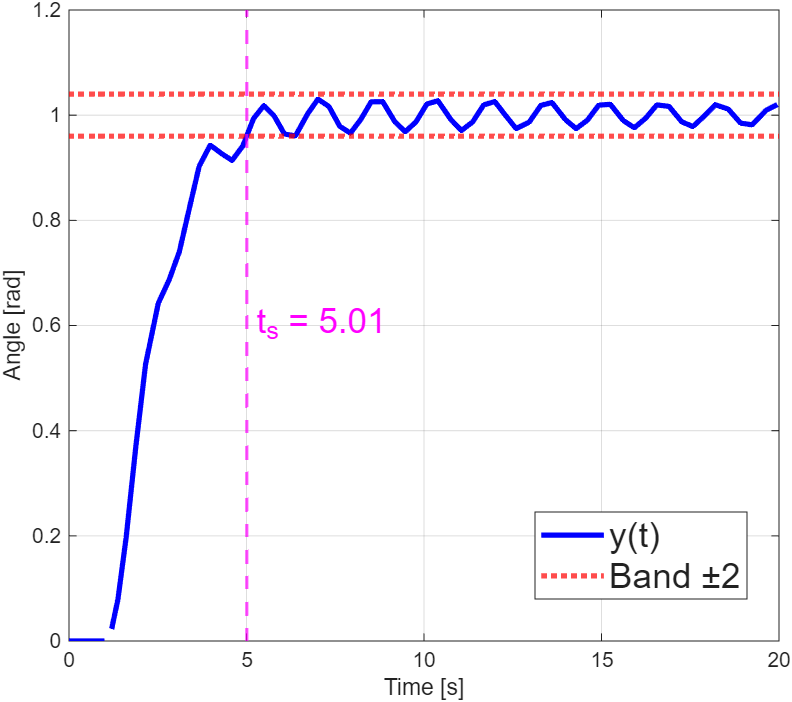
\includegraphics[width=0.35\textwidth]{Figures/simulation_PID.png}
  \caption{Simulated step response of the PID controller.}
  \label{fig:pid_sim}
\end{figure}

The experimental step response recorded on the physical platform. The out put enters and remains inside the  $\pm 2\%$ band with a small peak overshoot
before settling cleanly, as summarised in Table~\ref{tab:PID_metrics}. A disturbance injected
at $t = 20\,\text{s}$ causes a transient excursion, after which the controller successfully
rejects it and returns the output to the reference, demonstrating integral action and robustness
to step disturbances.

\begin{figure}[H]
  \centering
  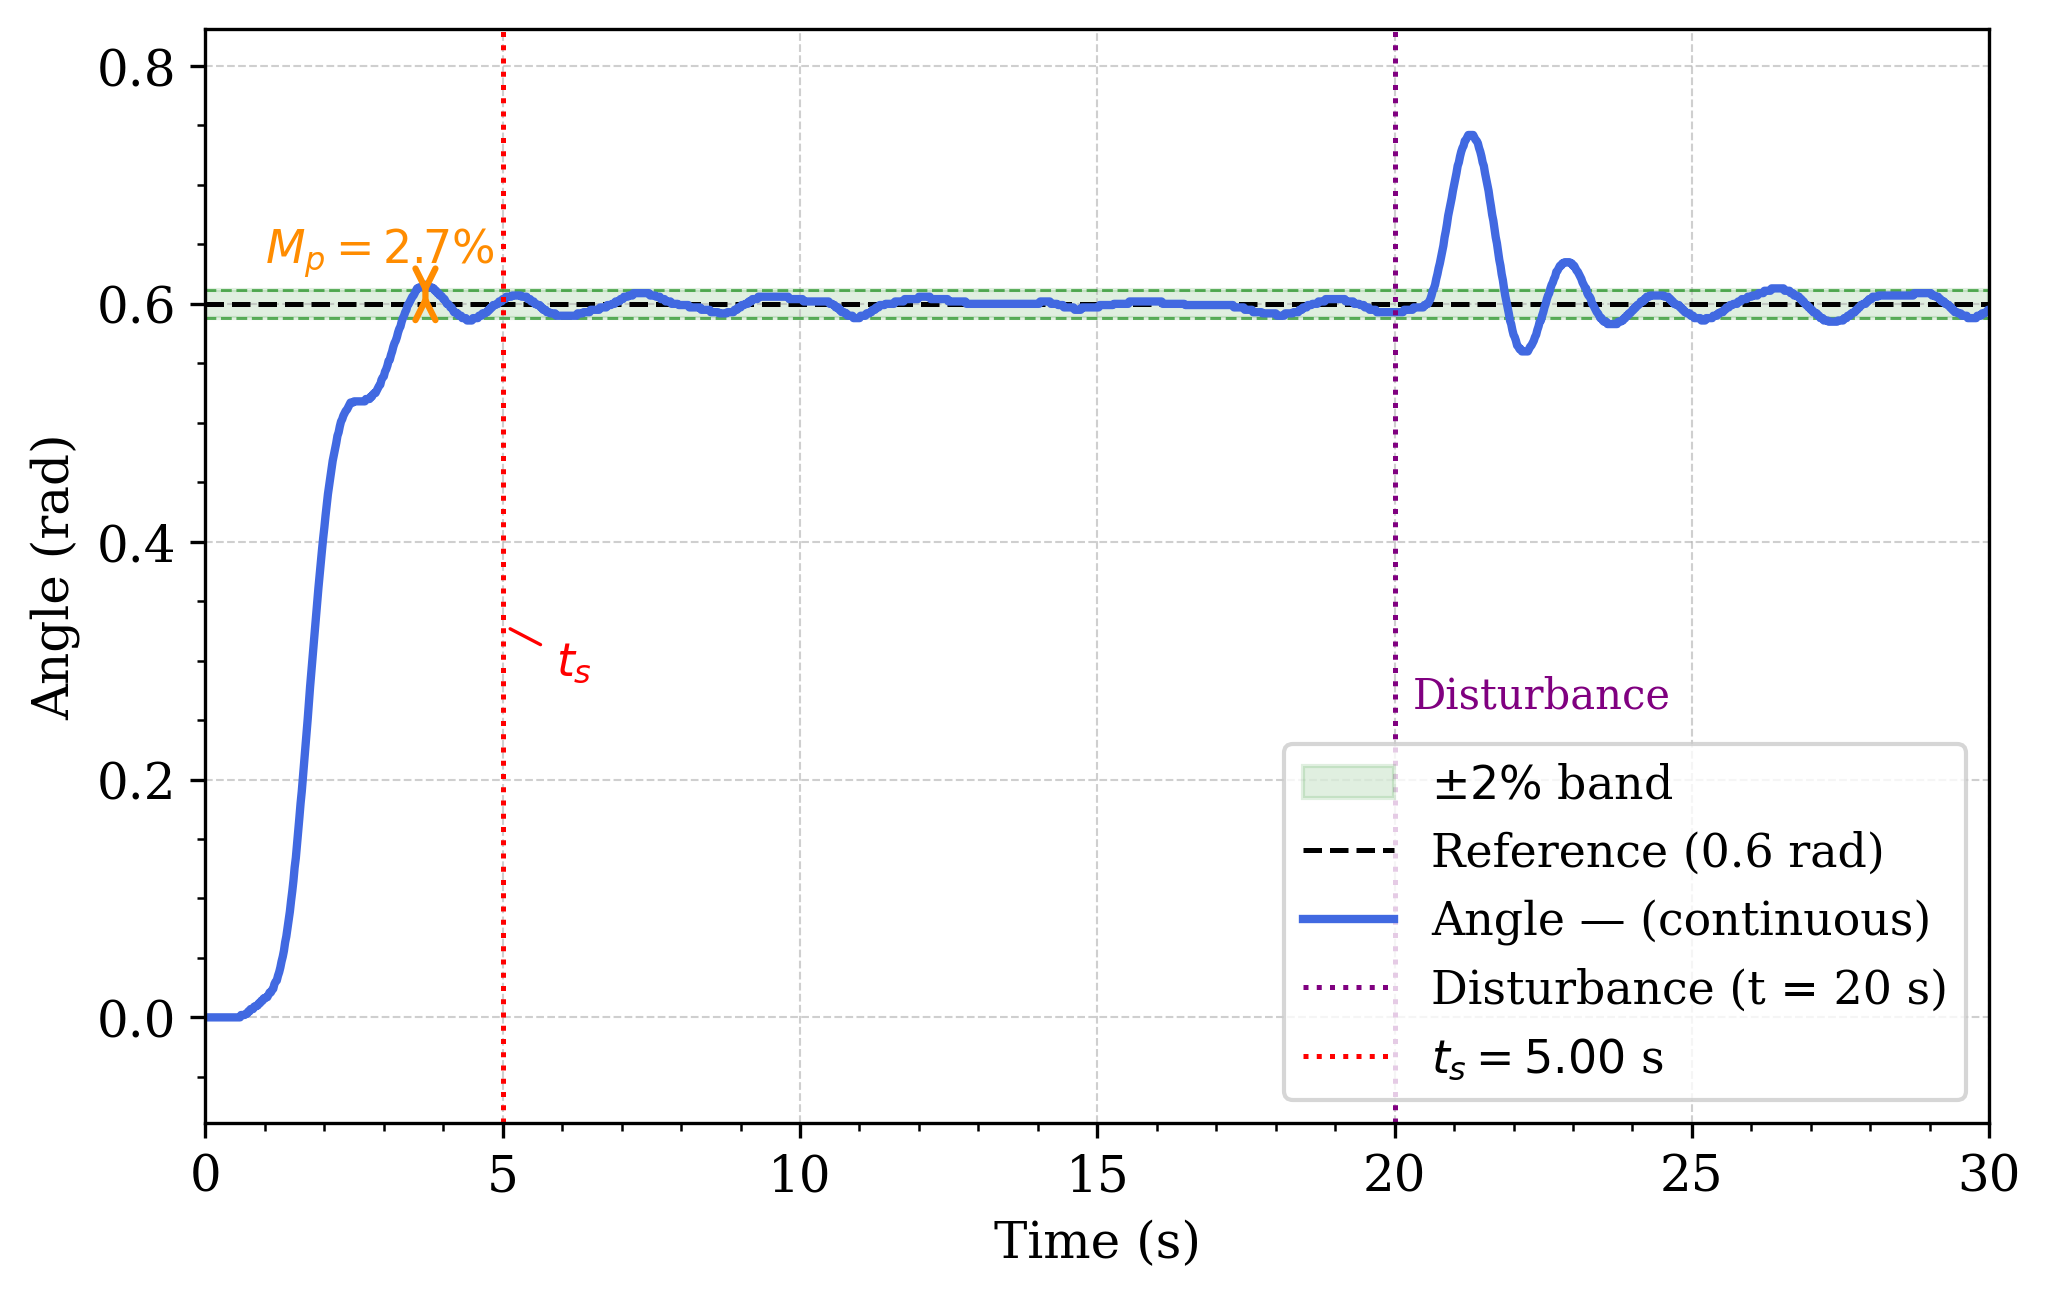
\includegraphics[width=0.45\textwidth]{Figures/experimental_pid.png}
  \caption{Experimental step response of the PID controller.}
  \label{fig:pid_exp}
\end{figure}

The primary difference between the two responses lies in the steady-state behaviour after
settling. In simulation, the output exhibits a sustained low-amplitude oscillation that keeps
it cycling inside the $\pm 2\%$ band, whereas experimentally the response damps out and
converges to the reference without visible oscillation. Furthermore, the experimental response
presents a visible peak overshoot before entering the band, a feature absent in the simulated
response.

To improve the experimental behaviour, the derivative filter coefficient was adjusted from
$N = 3$ to $N = 5$ while keeping $K_p$, $K_i$, and $K_d$ unchanged. Increasing $N$ raises
the filter cutoff frequency, allowing the derivative action to respond over a wider frequency
range. This produces a stronger damping effect on the real platform, which explains both the
suppression of the post-settling oscillation and the cleaner convergence observed experimentally.
On the real plant, the increased derivative
activity provided by $N = 5$ attenuates those higher-frequency components, resulting in a
smoother and more stable steady-state response.

\begin{table}[H]
  \centering
  \captionsetup{skip=4pt}
  \renewcommand{\arraystretch}{0.95}
  \caption{PID performance metrics: simulation vs.\ experiment}
  \begin{tabular}{lcccc}
    \toprule
    Condition    & $t_s$ (s) & $M_p$ (\%) & $e_{ss}$ & Meets specs? \\
    \midrule
    Simulation   & 5.01 & 3.4 & 0 & \textbf{No} \\
    Experimental & 5 & 2.7 & 0 & \textbf{Yes} \\
    \bottomrule
  \end{tabular}
  \label{tab:PID_metrics}
\end{table}

%------------------------------------------------
\subsection{Integral State Feedback Controller via LQR}

The closed-loop step responses of the ISF-LQR controller for $r = 0.6$~rad are shown in Fig.~1 (experiment) and Fig.~2 (simulation). The corresponding performance metrics are summarized in Table~\ref{tab:lqr_metrics}.

\begin{figure}[H]
  \centering
  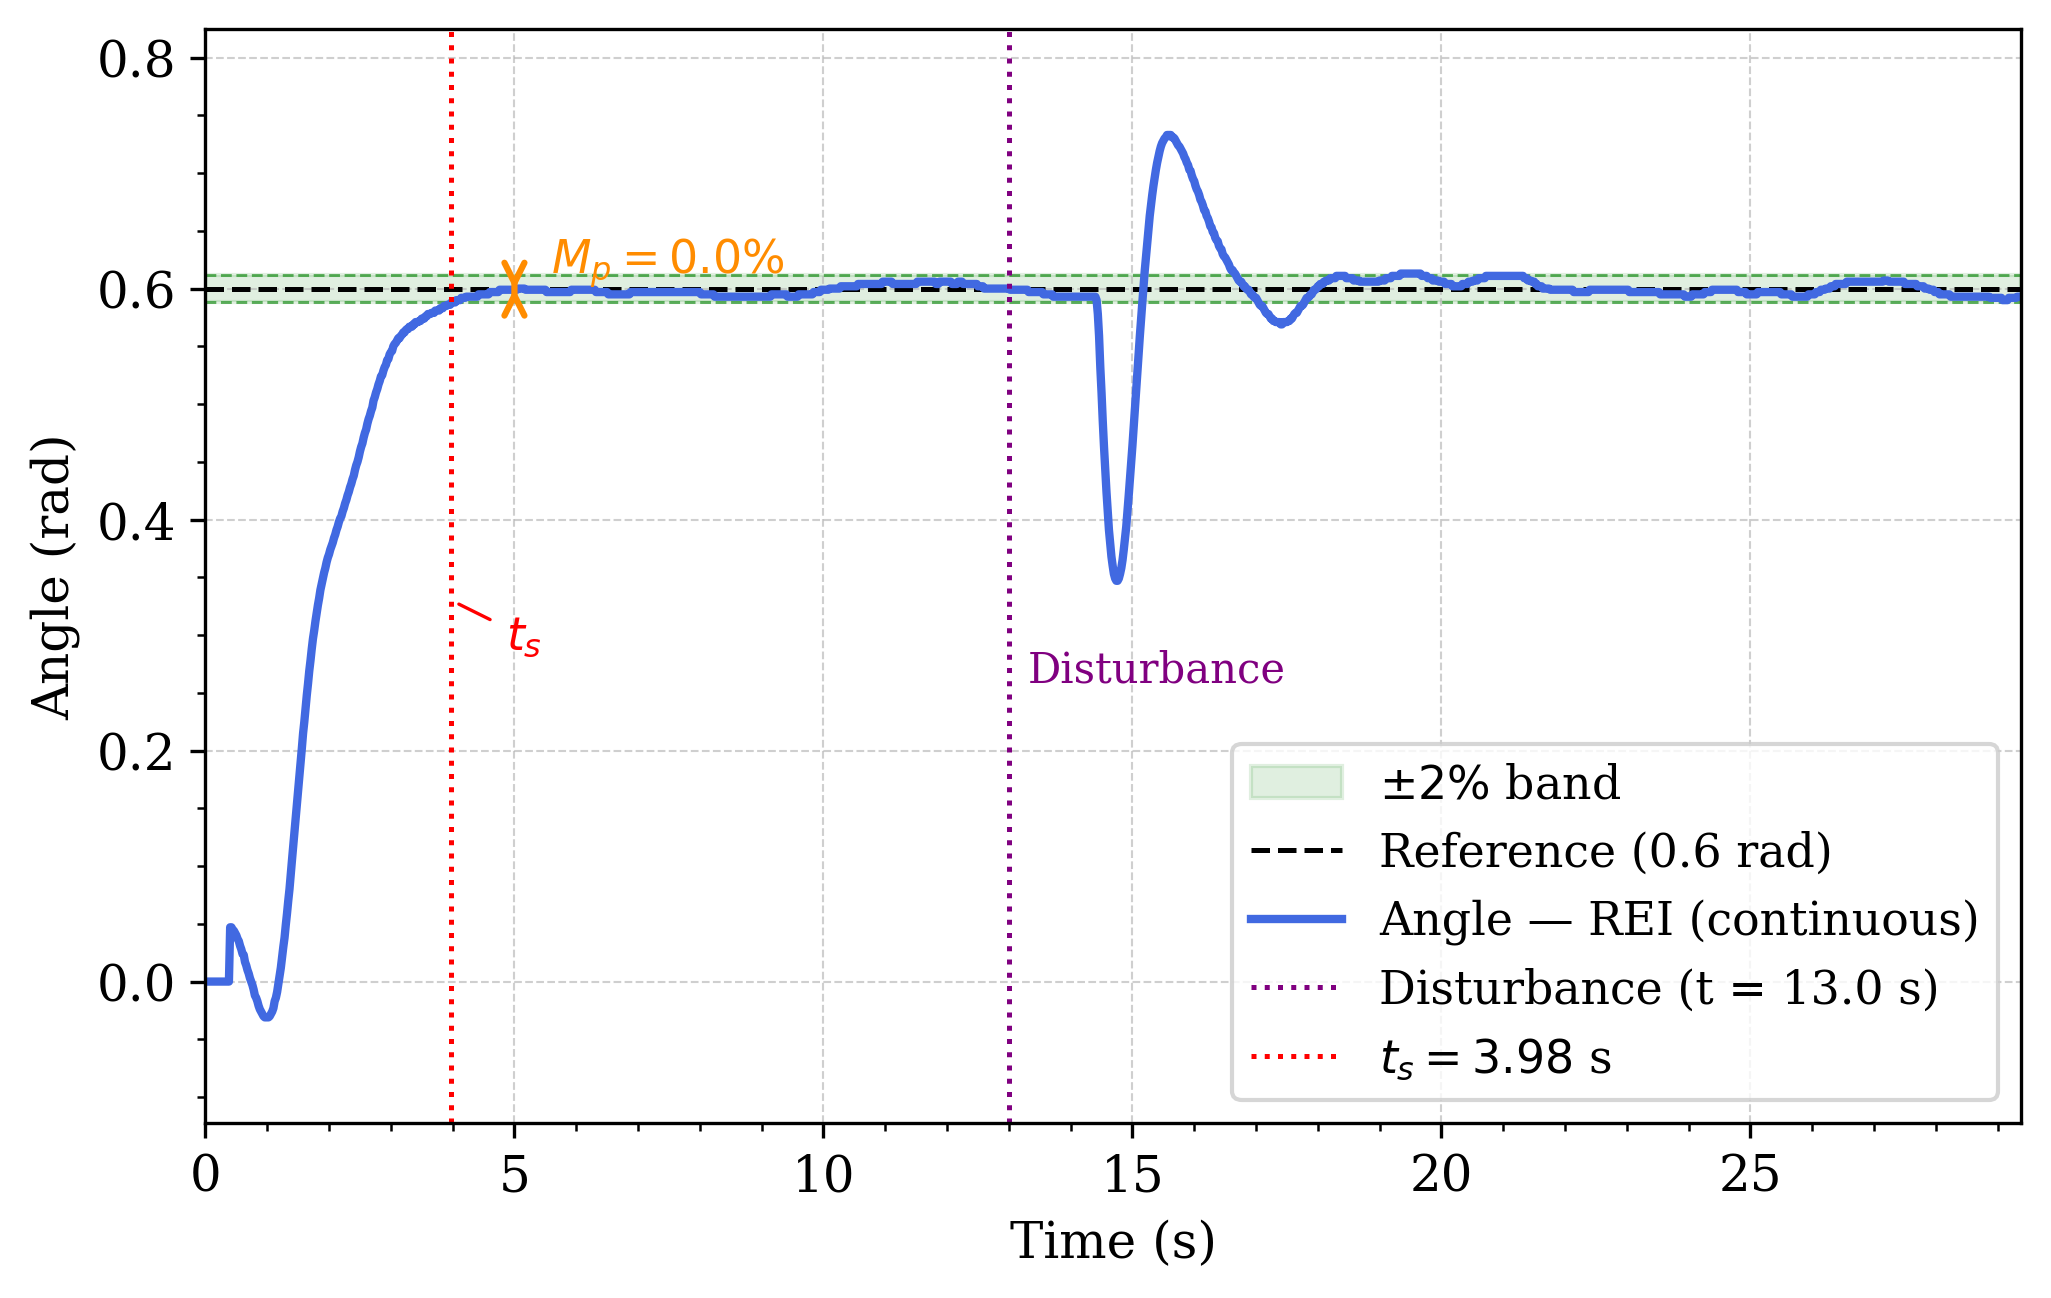
\includegraphics[width=0.45\textwidth]{Figures/experimental_rei.png}
  \caption{Experimental step response of the ISF-LQR controller.}
  \label{fig:lqr_exp}
\end{figure}

\begin{figure}[H]
  \centering
  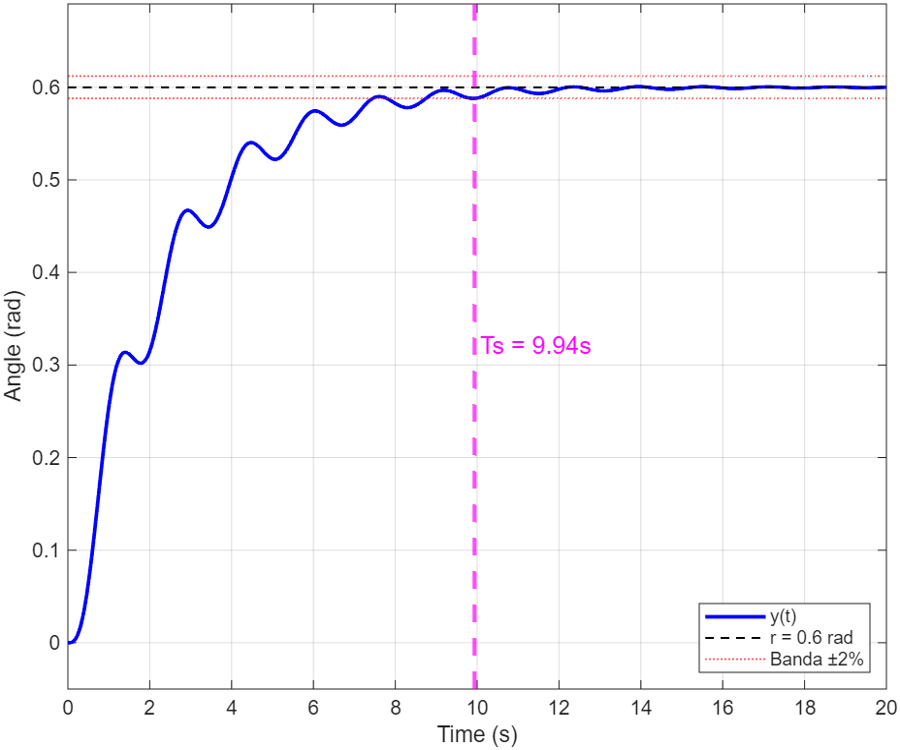
\includegraphics[width=0.35\textwidth]{Figures/simulation_rei.png}
  \caption{Simulated step response of the ISF-LQR controller.}
  \label{fig:lqr_sim}
\end{figure}

\begin{table}[H]
  \centering
  \caption{ISF-LQR performance metrics: simulation vs.\ experiment}
  \begin{tabular}{lcccc}
    \toprule
    Condition    & $t_s$ (s) & $M_p$ (\%) & $e_{ss}$ & Meets specs? \\
    \midrule
    Simulation   & 9.94 & 0.12 & 0 & \textbf{No} \\
    Experimental & 3.98 & 0    & 0 & \textbf{Yes} \\
    \bottomrule
  \end{tabular}
  \label{tab:lqr_metrics}
\end{table}

Both conditions satisfy $e_{ss}=0$ and $M_p \leq 3\%$;
the settling time discrepancy is addressed in
Section~V.
%------------------------------------------------

\subsection{I-PD Controller via Pole Placement}
The closed-loop step responses for the I-PD controller
are shown in Figs.~5 (experimental) and~6 (simulation).
Performance metrics are summarized in Table~VI.

% FIGURE 5 — experimental I-PD response
 \begin{figure}[h]
   \centering
	   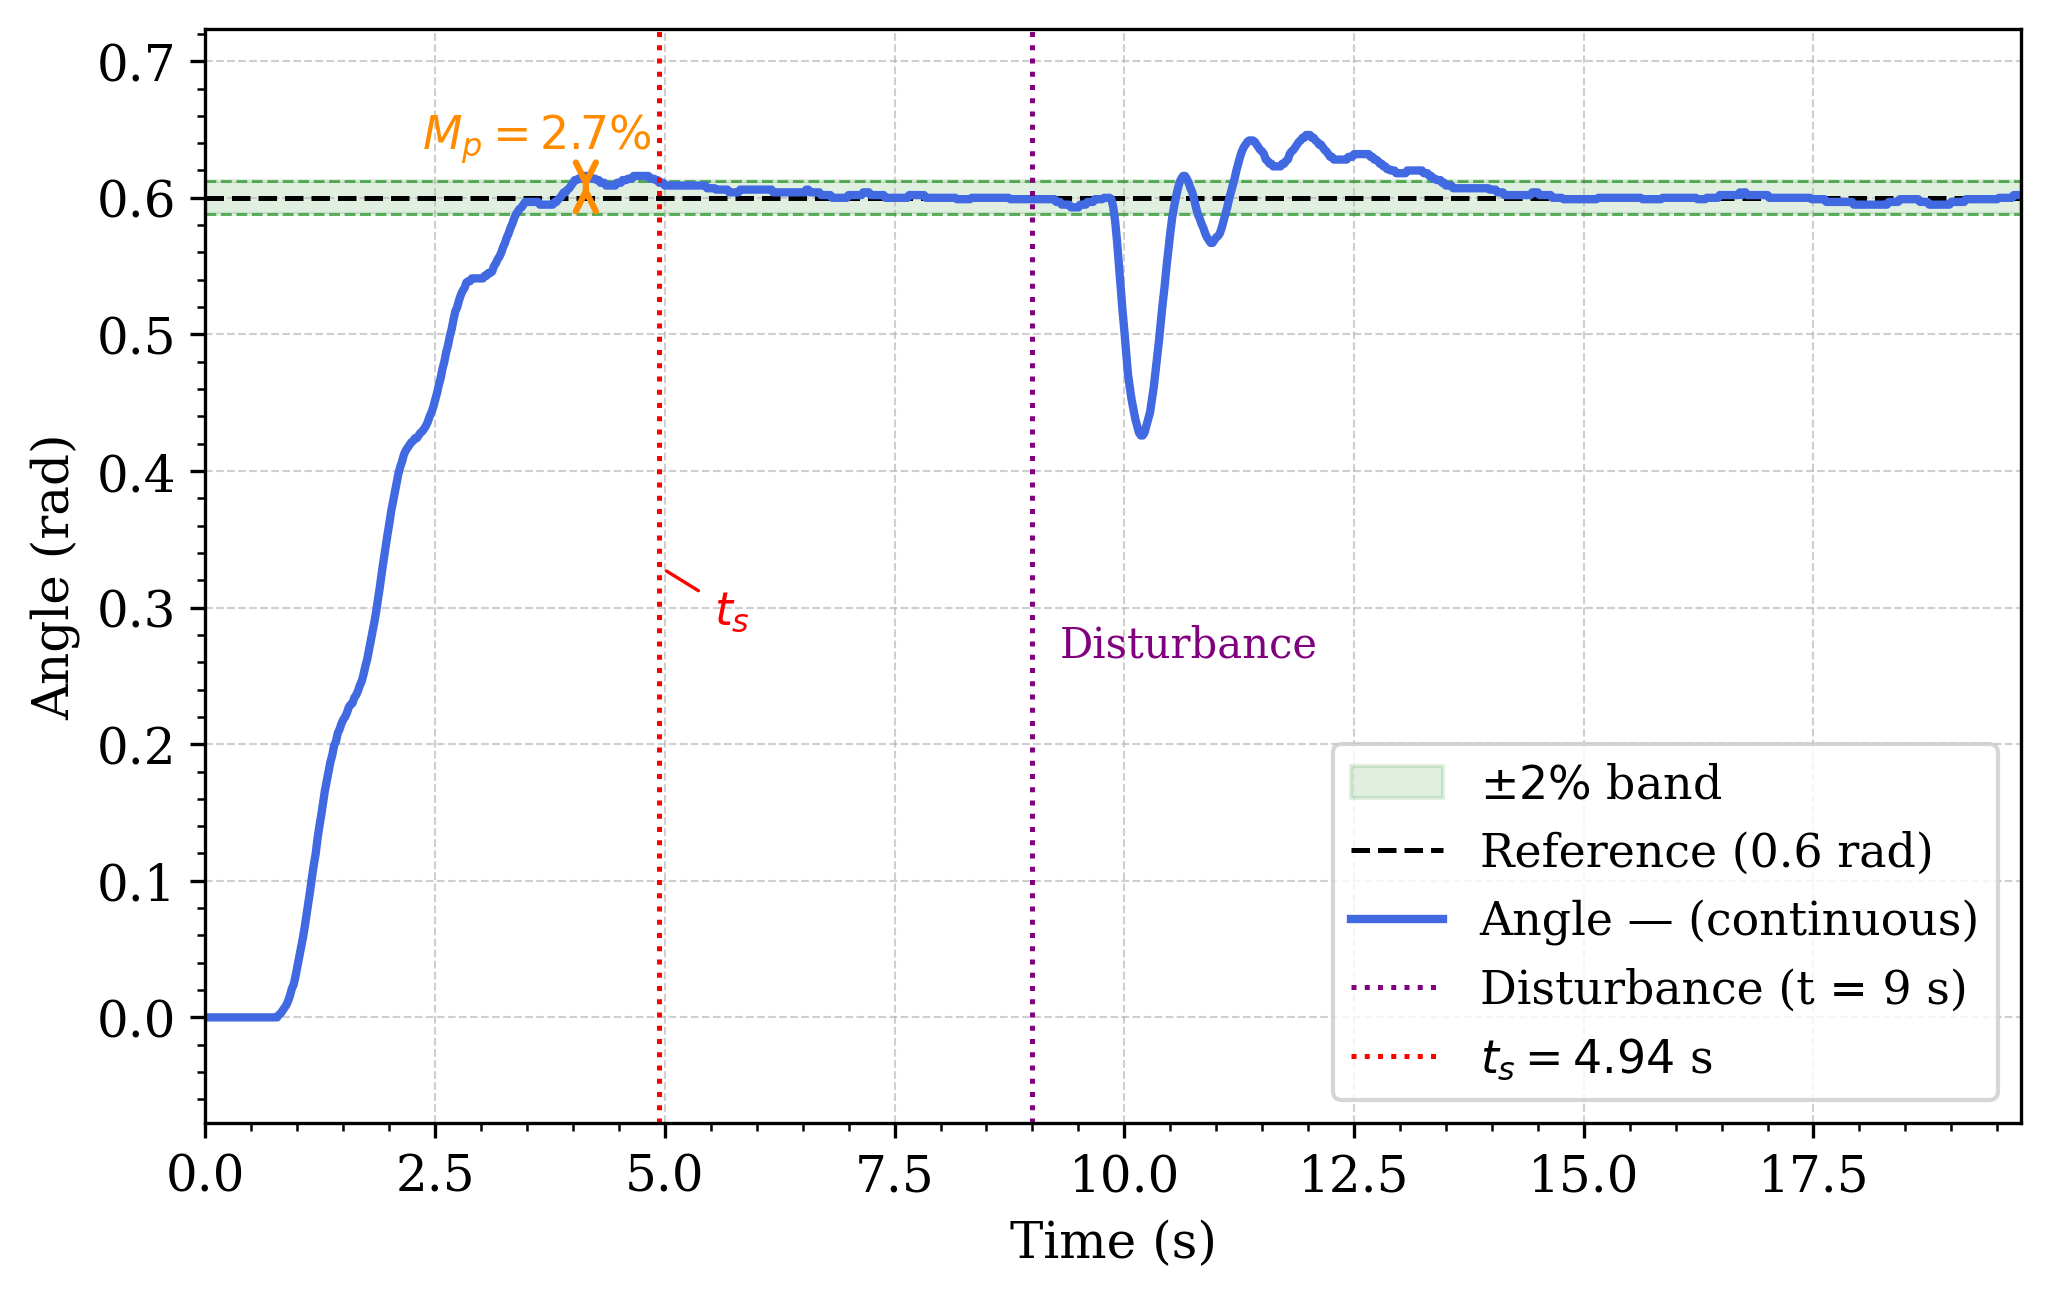
\includegraphics[width=0.45\textwidth]{Figures/experimental_ipd.png}
   \caption{Experimental step response of the I-PD controller.}
   \label{fig:ipd_exp}
 \end{figure}

 \begin{figure}[h]
   \centering
   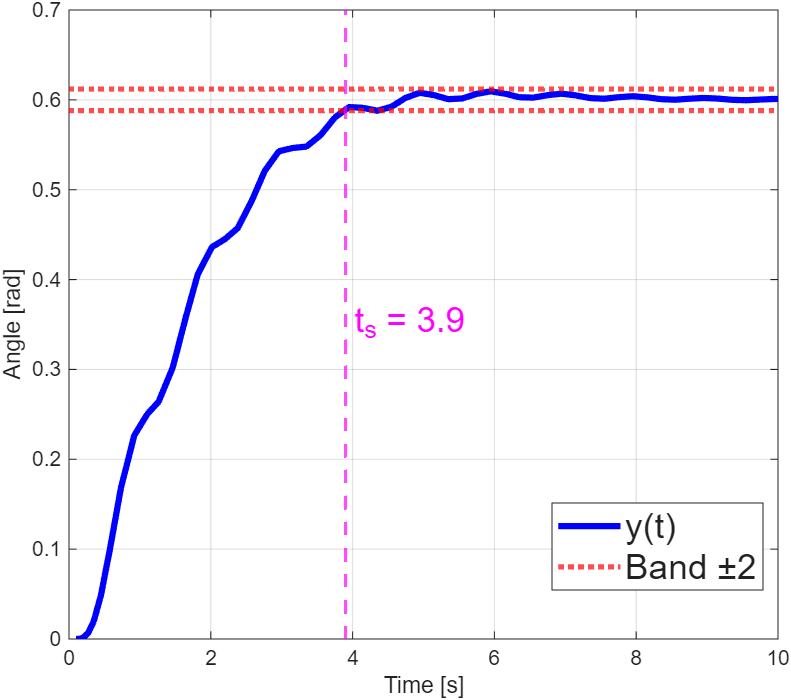
\includegraphics[width=0.35\textwidth]{Figures/simulation_IPD.png}
   \caption{Simulated step response of the I-PD controller.}
   \label{fig:ipd_sim}
 \end{figure}

The simulated response exhibits near-critically-damped
behaviour ($M_p = 1\%$, $t_s = 3.9$~s), consistent with
the chosen pole locations ($\zeta_d \approx 0.946$). The
actuator saturation included in simulation produces a
mild oscillatory entry visible in both curves, caused by
the motor saturating to zero when the pendulum exceeds
the reference, a physically inevitable consequence of
the unidirectional propeller thrust. Despite this, both
responses remain within specifications.

\begin{table}[h]
\centering
\caption{I-PD performance metrics: simulation vs. experiment}
\begin{tabular}{lcccc}
\toprule
Condition & $t_s$ (s) & $M_p$ (\%) & $e_{ss}$ & Meets specs? \\
\midrule
Simulation   & 3.9 & 1.0 & 0 & Yes \\
Experimental & 4.94 & 2.7 & 0 & Yes \\
\bottomrule
\end{tabular}
\label{tab:ipd}
\end{table}

%------------------------------------------------
\subsection{Discrete PID Controller}
% Add simulation and experimental results here.

% \begin{figure}[H]
%   \centering
%   \includegraphics[width=0.45\textwidth]{pid_disc_comp.png}
%   \caption{Discrete PID — simulated vs.\ experimental step response.}
%   \label{fig:pid_disc_comp}
% \end{figure}

The discrete PID controller \eqref{eq:pid_discrete}, designed via manual pole-zero placement,
failed to meet the imposed specifications on the physical plant. Unlike the continuous IMC
design, where the tuning parameter provides a structured and systematic path to
satisfy the closed-loop requirements, the manual approach is inherently sensitive to unmodelled
dynamics. In discrete time, this sensitivity is further amplified by quantisation effects
introduced by the sampling process, discretisation approximation errors in the derivative
action, and the reduced phase margin that results from the computational delay added by the
digital implementation. These factors, absent in the continuous design, cause the discrete
controller to behave differently on the real platform than predicted by the linear model.
Due to the unsatisfactory experimental outcome, no simulation or experimental plots are
included for this controller.
%------------------------------------------------
\subsection{Comparative Summary}
%-----------------------------------------------------------------
% SUGGESTED TABLE — overall simulated vs. experimental performance:
%
% \begin{table}[H]
%   \centering
%   \caption{Performance metrics comparison (simulation vs.\ experimental)}
%   \begin{tabular}{llcccc}
%     \toprule
%     Controller      & Condition    & $t_s$ (s) & $M_p$ (\%) & $e_{ss}$ & Meets specs? \\
%     \midrule
%     Continuous PID  & Simulation   & ... & ... & ... & Yes/No \\
%                     & Experimental & ... & ... & ... & Yes/No \\
%     \midrule
%     ISF-LQR         & Simulation   & 9.94 & 0.12 & 0 & No \\
%                     & Experimental & 3.98 & 0    & 0 & Yes \\
%     \midrule
%     I-PD            & Simulation   & ... & ... & ... & Yes/No \\
%                     & Experimental & ... & ... & ... & Yes/No \\
%     \midrule
%     Discrete PID    & Simulation   & ... & ... & ... & Yes/No \\
%                     & Experimental & ... & ... & ... & Yes/No \\
%     \bottomrule
%   \end{tabular}
%   \label{tab:comparison}
% \end{table}
% -----------------------------------------------------------------

%================================================
%  5. DISCUSSION
%================================================
\section{Discussion}
\label{sec:disc}
% -----------------------------------------------------------------
% WHAT TO WRITE HERE:
%   • Interpret (do not repeat) the results from the previous section.
%   • Explain discrepancies between simulation and experiment:
%     nonlinearities, friction, actuator dead zone, time delay.
%   • Analyze why one controller outperforms the others in terms
%     of robustness or ease of tuning.
%   • Relate the rejection of sample 3 to the importance of data
%     quality in system identification.
%   • Discuss the impact of the sampling period on the discrete PID.
%   • Point out limitations of the linear 2nd-order model versus
%     the actual PADP behavior.
%   • Propose improvements: state observer, adaptive control,
%     higher sensor resolution, etc.
% -----------------------------------------------------------------
This section interprets the results presented above, analyzing the causes of the observed differences between theoretical models and the physical behavior of the system, as well as the advantages and disadvantages of each implemented control strategy.

%------------------------------------------------
\subsection{ISF-LQR: Simulation--Experiment Discrepancy}

Figs.~\ref{fig:lqr_sim} and~\ref{fig:lqr_exp} show a clear contrast between simulated and experimental responses. The simulation exhibits a slowly damped transient with $t_s = 9.94$~s, consistent with the real pole $p_3 = -0.4509$ near the imaginary axis, which dominates the settling behavior despite the faster complex poles. In contrast, the experimental response converges monotonically to the 0.6~rad reference in $t_s = 3.98$~s with zero overshoot, satisfying both specifications.

A small negative deflection at $t \approx 1$~s in the experimental response (about $-0.07$~rad) is attributed to actuator dead-zone and propeller inertia, which delay the onset of effective control action. This effect is not captured by the linear model.

The faster experimental convergence is consistent with additional nonlinear damping (e.g., friction and aerodynamic drag), which increases the effective damping and suppresses oscillations, leading to a shorter settling time than predicted.

Finally, the experimental response shows effective disturbance rejection; a perturbation at $t \approx 13$~s produces a deviation of approximately 0.25~rad, after which the output returns to the reference, remaining within the margin of less than $2\%$ steady-state error. This confirms the role of comprehensive action in rejecting disturbances despite the model's inaccuracies.

% -----------------------------------------------------------------
% Add discussion for remaining controllers below:
%   • Continuous PID: comment on SISOtool tuning conservativeness
%   • I-PD: pole placement vs. LQR trade-offs
%   • Discrete PID: impact of sampling period, quantization effects
% -----------------------------------------------------------------

%================================================
%  6. CONCLUSIONS
%================================================
\section{Conclusions}
% -----------------------------------------------------------------
% WHAT TO WRITE HERE:
%   • Summarize the main achievements (successful identification,
%     number of controllers that met the specifications).
%   • State which controller proved most suitable and why
%     (performance, implementation ease, robustness).
%   • Mention the challenges encountered (disturbance in sample 3,
%     simulation–experiment discrepancies).
%   • Reflect on the methodological learning of the project
%     (complete cycle: data → model → control → validation).
%   • Propose future work: nonlinear control, cascade control,
%     active disturbance rejection, etc.
% -----------------------------------------------------------------
The ISF-LQR controller achieved zero steady-state error and effective disturbance rejection. While the simulation resulted in $t_s = 9.94$~s and $M_p = 0.12\,\%$, failing the settling time requirement, the experimental response reached $t_s = 3.98$~s with $M_p = 0\,\%$, satisfying all specifications.
%================================================
%  REFERENCES
%================================================
\begin{thebibliography}{9}

\bibitem{ogata2010}
K.~Ogata, \textit{Modern Control Engineering}, 5th~ed.
Prentice Hall, 2010.

\bibitem{ljung1999}
L.~Ljung, \textit{System Identification: Theory for the User}, 2nd~ed.
Prentice Hall, 1999.

\bibitem{astrom2006}
K.~J.~Åström and T.~Hägglund, \textit{Advanced PID Control}.
ISA, 2006.

\bibitem{anderson1990}
B.~D.~O.~Anderson and J.~B.~Moore, \textit{Optimal Control: Linear
Quadratic Methods}.
Prentice Hall, 1990.

\bibitem{visioli2006}
A.~Visioli, \textit{Practical PID Control}.
Springer, 2006.

\bibitem{franklin1998}
G.~F.~Franklin, J.~D.~Powell, and M.~L.~Emami-Naeini,
\textit{Feedback Control of Dynamic Systems}, 4th~ed.
Prentice Hall, 1998.

\end{thebibliography}

%================================================
\end{document}